\chapter{Methodology}
\label{ch:methodology}

\section{PulseDB Dataset}

This thesis uses PulseDB, a large cleaned dataset built from MIMIC-III \citep{mimic2016} and VitalDB \citep{vitaldb2022}, designed for benchmarking cuffless BP estimation methods under standardised testing protocols \citep{pulsedb2023}. Each record contains synchronised PPG, ECG, and arterial BP signals sampled at 125 Hz, segmented into 10-second windows with reference systolic blood pressure (SBP) and diastolic blood pressure (DBP) labels. The complete PulseDB comprises 5,361 subject records --- 2,423 from the MIMIC-III subset and 2,938 from the VitalDB subset --- totalling 5.24 million segments. This thesis uses the complete dataset, yielding 5,159 subject records and 5.23 million valid PPG segments after quality gating and feature extraction.

Two properties of the source distribution should be noted. First, the two subsets reuse the same \texttt{p}\textit{NNNNNN}\texttt{.mat} filename convention, so 339 filenames occur in both; because subject identity is keyed on the source filename, these pairs are merged into a single record, which is why 5,361 source files reduce to 5,159 subject keys. Second, an initial extraction pass double-counted 319,361 segments (5.75\%) that were present in a duplicated copy of the source directories; these were removed by de-duplicating on segment identifier. Neither issue affects the reported results: every duplicated segment carries the same subject key and therefore falls within a single split, and an audit of the evaluation confirmed that the 25 segments used per test subject always originate from one source file.

\subsection{Signal Preprocessing}

A five-stage preprocessing pipeline is applied: (1) quality gating to reject motion artefacts; (2) baseline drift removal via high-pass filtering; (3) power-line noise suppression; (4) band-pass filtering at 0.5--8 Hz; (5) flat-line detection.

\subsection{Peak and Fiducial Point Detection}

A dual-strategy approach detects PPG peaks and fiducial points \citep{pyppg2024}: a derivative-based detector for systolic peaks, and a landmark-based detector for the dicrotic notch and diastolic onset.

\section{Multi-Dimensional Feature Engineering}

A total of 55 features are extracted from each 10-second PPG segment, organised into four categories following feature sets established in the cuffless BP estimation literature \citep{elgendi2012,liang2018,slapnicar2019}. Age and gender are additionally included as demographic features. Table~\ref{tab:features} summarises the feature taxonomy.

\begin{table}[htbp]
\centering
\caption{The 55-dimensional PPG feature set extracted from each 10-second segment.}
\label{tab:features}
\small
\begin{tabular}{l c p{9.5cm}}
\toprule
Category & Dim. & Representative features \\
\midrule
Time-domain morphology & 16 & systolic/diastolic amplitudes, pulse amplitude, heart rate, pulse interval, upstroke time, diastolic time, pulse widths at 25/50/75\% height, augmentation index (AIx), stiffness index (SI) \\
Derivative morphology (VPG + APG) & 18 & VPG max/min/std/mean-abs; APG a--e wave means and stds; b/a, c/a, d/a, e/a ratios \\
Global statistics & 14 & mean, std, median, skewness, kurtosis, min/max, peak-to-peak, RMS, percentiles (p5/p25/p75/p95), entropy \\
Frequency domain & 7 & spectral energy, HR band power and ratio, dominant frequency and power, spectral centroid, LF/HF ratio \\
\midrule
Total & 55 & \\
\bottomrule
\end{tabular}
\end{table}

Figure~\ref{fig:fiducial_points} illustrates the fiducial points detected on a single PPG pulse and the principal time-domain features derived from them.

\begin{figure}[htbp]
\centering
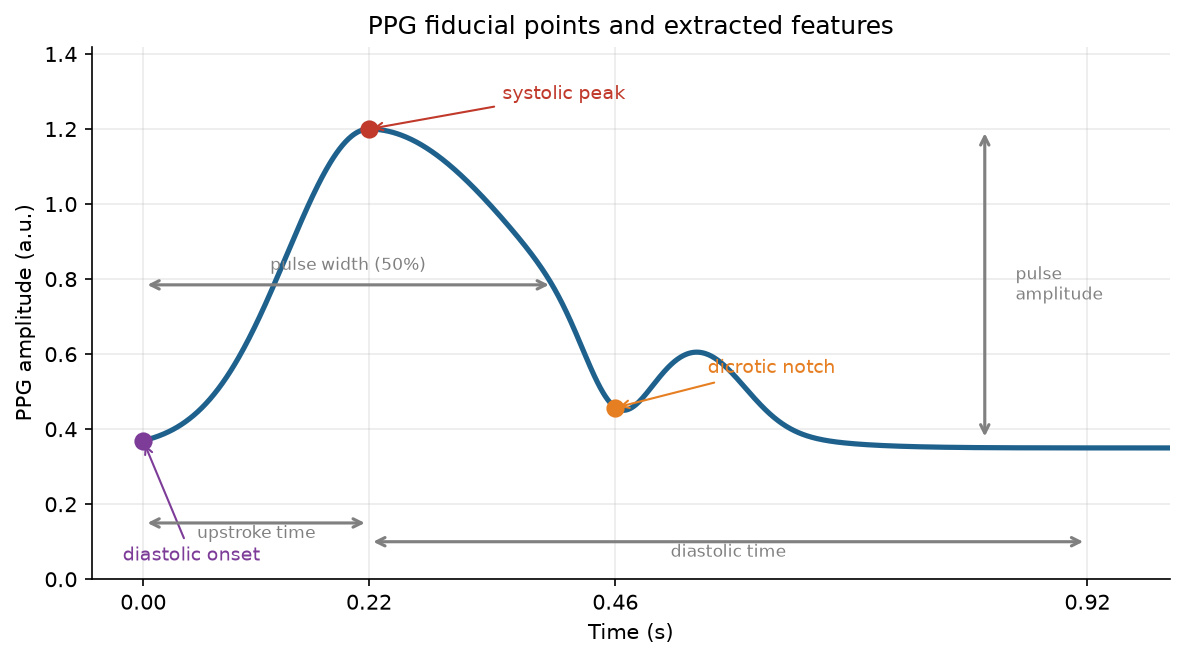
\includegraphics[width=0.85\textwidth]{figures/fig_fiducial_points.png}
\caption{Fiducial points detected on a single PPG pulse (systolic peak, dicrotic notch, diastolic onset) and the time-domain features derived from them: pulse amplitude, upstroke time, pulse width at 50\% height, and diastolic time.}
\label{fig:fiducial_points}
\end{figure}

\textbf{Time-domain features} (16) characterise cardiac timing and waveform morphology. Systolic-peak and diastolic-onset amplitudes yield the systolic amplitude mean/std, diastolic amplitude mean and pulse amplitude; inter-beat intervals give the pulse-interval mean/std and heart rate ($60{,}000/\overline{PPI}$). Systolic upstroke time and diastolic time reflect ejection speed and peripheral resistance. Pulse widths measured at 25\%, 50\% and 75\% of pulse height capture arterial compliance. Two derived indices are included: the augmentation index (\texttt{aix}), the ratio of reflected to forward wave amplitude indicative of arterial stiffness, and the large-artery stiffness index (\texttt{stiffness\_index}), defined as pulse interval divided by upstroke time.

\textbf{Derivative features} (18) are computed from the first derivative (velocity plethysmogram, VPG) and the second derivative (acceleration plethysmogram, APG). Four VPG statistics (\texttt{vpg\_max}, \texttt{vpg\_min}, \texttt{vpg\_std}, \texttt{vpg\_mean\_abs}) quantify the rate of blood-volume change. Per-beat APG analysis extracts the amplitudes of the five characteristic waves (a--e): five means, five standard deviations, and the four ratios \texttt{apg\_b\_a\_ratio}, \texttt{apg\_c\_a\_ratio}, \texttt{apg\_d\_a\_ratio} and \texttt{apg\_e\_a\_ratio}. The b/a ratio is a classical marker of vascular ageing, while c/a relates to arterial-wall viscoelasticity \citep{elgendi2012}.

\textbf{Statistical features} (14) are computed over the whole segment independently of beat detection, providing robustness to peak-detection errors: mean, standard deviation, median, skewness, kurtosis, minimum, maximum, peak-to-peak amplitude, RMS, the 5/25/75/95 percentiles and histogram-based entropy (\texttt{ppg\_entropy}).

\textbf{Frequency-domain features} (7) are derived via fast Fourier transform (FFT): total spectral energy, heart-rate band power (0.5--5 Hz) and its ratio to total power, dominant frequency and its power, spectral centroid, and the LF/HF ratio (0--0.5 Hz vs.\ 0.5--5 Hz).

\section{Evaluation Protocol}

\subsection{Problem Formulation}

BP estimation is a multi-output regression: given N training samples $\{(\mathbf{x}_i, y_i^{SBP}, y_i^{DBP})\}$, learn mappings $f_{SBP}(\mathbf{x})$ and $f_{DBP}(\mathbf{x})$ minimising test-set error.

\subsection{Subject-Level vs Segment-Level Splits}

Two evaluation protocols are distinguished. \textbf{Segment-level split} randomly shuffles all segments, allowing same-subject leakage and inflated accuracy. \textbf{Subject-level split} ensures no test subject appears in training --- the only correct way to evaluate cross-subject generalisation.

\subsection{Calibration Protocol}

For personalised calibration, the first K chronological segments are used of each test subject as calibration samples (K $\in \{1,3,5,10,20\}$), and the subsequent 5 segments for testing. This reflects real deployment, where calibration data arrives chronologically.

\section{Traditional ML Baseline}

Under the strict 70/20/10 subject-level split (3,611 training / 1,031 validation / 517 held-out test subjects), XGBoost is trained \citep{chen2016xgboost} (300 trees, max depth 6, learning rate 0.05) on the 3,611 training subjects. The result on the 517 test subjects is SBP MAE = 15.7 mmHg, DBP MAE = 8.89 mmHg --- far from clinical usability (British Hypertension Society (BHS) Grade A requires $\leq$5 mmHg). This confirms the fundamental difficulty of cross-subject BP estimation, evaluated against the BHS protocol \citep{bhs1993} and IEEE wearable cuffless standard \citep{ieee1708}.

For fair comparison with LLM few-shot calibration, two conventional ML K-calibration methods are also implemented ML K-calibration methods: \textbf{bias correction} (global prediction plus the mean residual on K calibration samples) and \textbf{fine-tuning} (global model further trained on K samples).

\section{Models and Inference}

\textbf{LLM}: Qwen3-8B \citep{qwen3_2025}, run locally on an NVIDIA A100-80GB GPU. Each 10-second PPG segment (1,250 samples at 125 Hz) is reduced to 55 numerical features, which are then rendered as text --- either raw numbers or semantic clinical descriptions --- and tokenised by the LLM's tokenizer into token IDs before generation. Thinking mode is disabled (\texttt{enable\_thinking=False}), with greedy decoding and max 64 new tokens. Output parsing preferentially matches \texttt{SBP=}/\texttt{DBP=} labels.

\textbf{Semantic description}: the 55 numerical features are translated into a three-level clinical narrative by rule-based mappings derived from cardiovascular physiology, while \emph{retaining quantitative anchors}. The \emph{statistical level} reports raw vital measurements directly (heart rate, pulse interval, pulse width); the \emph{structural level} reports waveform-morphology quantities as numbers (APG wave ratios, PPG skewness and kurtosis); and the \emph{semantic level} maps the most physiologically decisive features to qualitative clinical interpretations using explicit thresholds. For example, the augmentation index is interpreted as low arterial stiffness (AIx $<$ 60\%), moderate (60--80\%), or high ($>$ 80\%); the APG b/a ratio as low ($< -0.4$), normal ($-0.4$ to $-0.2$), or high ($> -0.2$) vascular resistance; and heart rate as bradycardia ($<$ 60 bpm), normal (60--100), or tachycardia ($>$ 100). Every semantic phrase retains its quantitative anchor in parentheses, so no information is lost.

A complete description has the form:

\begin{quote}
\small
[Statistical] heart rate 72.5 bpm; pulse interval 827.6 ms; pulse width 280.0 ms\\
[Structural] APG b/a ratio $-0.350$; APG c/a ratio $0.100$; systolic amplitude $1.200$; PPG skewness $0.30$; PPG kurtosis $3.50$\\
[Semantic] normal heart rate (HR 72 bpm); moderate arterial stiffness (AIx 75\%); normal vascular resistance (b/a $-0.35$); moderate arteries (stiffness 7.2); normal contractility (upstroke 180 ms)
\end{quote}

The thresholds are taken from standard cardiovascular reference ranges rather than tuned on the data, so the mapping is transparent and clinically interpretable. The semantic description is generated deterministically from the same 55 features as the numeric prompt; the only difference between the two conditions is the representation of the input.

\textbf{Semantic bottleneck}: the LLM first generates a purely qualitative summary discarding all numbers, then predicts BP from the summary alone.
